\documentclass[11pt,final,oneside]{fithesis}
\usepackage[utf8]{inputenc}
\usepackage[T1]{fontenc}
\usepackage{tipa}
\usepackage[slovak]{babel}
\usepackage{tabularx}
\usepackage{graphicx}
\usepackage{cite}
\usepackage{url}

\hbadness=1000
\tolerance=1000

\newcommand{\smalltt}[1]{\small\texttt{#1}\normalsize}

\thesistitle{Monitorování zátěže a využití výpočetních zdrojů v heterogenním výpočetním prostředí}
\thesissubtitle{Diplomová práca}
\thesisstudent{Juraj Leždík}
\thesiswoman{false}
\thesisfaculty{fi}
\thesisyear{jar 2016}
\thesisadvisor{Mgr. Miroslav Ruda}
\thesislang{sk}
\begin{document}

\FrontMatter
\ThesisTitlePage

\begin{ThesisDeclaration}
\DeclarationText
\AdvisorName
\end{ThesisDeclaration}


\begin{ThesisThanks}
\end{ThesisThanks}

\begin{ThesisAbstract}
\end{ThesisAbstract}

\begin{ThesisKeyWords}
\end{ThesisKeyWords}

\tableofcontents
\addcontentsline{toc}{chapter}{Obsah}

\MainMatter
\chapter{Úvod}
Cloudová infraštruktúra MetaCentra poskytuje výpočetné prostriedky pre mnohé vedecké a výskumné organizácie. Spracovávajú sa v nej veľké objemy dát. Je tvorená mnohými uzlami rozmiestnenými naprieč celou
Českou republikou. Podstatou fungovania cloudového modelu je zdieľanie veľkého výpočetného výkonu viacerými subjektami, pre ktoré by zabezpečenie vlastnej infraštruktúry predstavovalo neúmernú 
ekonomickú, personálnu a prevádzkovú záťaž. Princípom zdieľania je, že prostriedky by mali byť ideálne využívané všetkými rovnako. Nemalo by dochádzať k tomu, že jeden klient vyťaží cloud natoľko, že 
výpočetné úlohy ostatných dostanú nepomerne malý priestor. To je možné docieliť monitorovaním využitia výpočtového výkonu a periférií. Ak máme informácie o tom, kto koľko využíval zdroje, je možné
tot využívanie účtovať a zároveň do budúcnosti primerane obmedzovať. 

Aby bolo možné správne vyvodzovať závery o zaťažení cloudu, je potrebné zberať údaje o tom periodicky a kontinuálne v čase. Je potrebné sledovať parametre v pravidelných intervaloch. Každému intervalu 
prináleží hodnota, ktorá vypovedá o využití prostriedkov v danom momente. Takéto dáta sa nazývajú časové rady. Cloud zahŕňa množstvo uzlov, kde na každom môže byť spustených množstvo úloh. O každej je
potrebné zberať viacero parametrov - vyťaženie procesora, pamäte, periférií. To predstavuje veľké množstvo metrických údajov, ktoré je potrebné ukladať a nejakým spôsobom vyhodnocovať. Slúžia na to 
databázy časových rád. Účtovanie sa tiež deje v určitých pravidelných intervaloch. Je preto potrebné mať možnosť spätne dohľadať údaje o využívaní zdrojov. Uchovávať podrobné metrické dáta má výnzam na určité
obdobie. Nie je potrebné vedieť ako bol využívaný cloud úlohou pred piatimi rokmi každých päť sekúnd. Okrem toho by to predstavovalo veľké požiadavky na úložné kapacity, ktoré by rástli lineárne vzhľadom
na počet úloh a čas. Je preto žiaduce po nejakej dobe dáta agregovať do väčších celkov a tiež mazať už nazbierané podrobné časové rady.

Aby boli monitorovacie údaje spoľahlivé, je potrebné zabezpečiť periodický zber metrických údajov. Monitorovanie sa uskutočňuje pravidelným pýtaním sa na vyťaženie daného zdroja. Aplikácia, ktorá zdroj
využíva, vytvorí odpoveď a pošle ju späť monitorovacej aplikácií. Problém nastáva, ak odpoveď nie je vytvorená v dostatočne krátkom intervale. Povedzme, že chcem zberať údaje každých päť sekúnd. Aplikácia,
ktorá práve rieši úlohy ale môže byť plne zaneprázdená a nebude odpovedať na výzvy na údaje o vyťaženosti. Tento problém je potrebné riešiť. Ak k tomu dôjde, nemali by byť vytvárané ďalšie výzvy na túto
zaneprázdnenú aplikáciu v takej miere, ako keď plynulo odpovedala. Monitorovacia aplikácia by si mala zapamätať poslednú nameranú hodnotu a tú odoslať ako aktuálnu. Zároveň by sa mala zaneprázdnenej aplikácií
pýtať v menej častých intervaloch. Ak aplikácia začne odpovedať, všetko je v poriadku. Ak nie, je možné reagovať reštartovaním monitorovacej aplikácie. Ak ani táto reakcia problém nevyrieši, komplikácia 
nastala zrejme v dotazovanej aplikácií.

Cloud predstavuje heterogénnu infraštruktúru. Na reišenie výpočetných úloh sa použivajú rôzne technológie a aplikácie. Rôzne aplikácie pristupujú k výpočetným problém odlišnými postupmi. Všetky úlohy 
sú ale počítané na akoby jednom veľkom a veľmi výkonnom počítači. Tieto aplikácie teda používajú spoločné zdroje. Metrické dáta, ktoré budem zberať, by takisto mali vypovedať o vyťažení tých istých druhov 
zdrojov. Je preto potrebné identifikovať, ktoré metrické dáta z jednej aplikácie je možné porovnať s údajmi z inej aplikácie. Takto môžeme dostať celkový obraz o tom, ako rôzne technológie využívajú
jednu skupinu zdrojov a len takto je možné vzájomne tieto technológie zrovnávať a účtovať ich využitie. 





\\a
\\a
\\a
\\a
\\a

Toto už je ten pôvodný úvod

V súčasnosti sú informačné technológie rozšírené vo všetkých oblastiach nášho života. Používame jednoúčelové integrované obvody v elektrospotrebičoch a predmetoch dennej, ako napr. v automatickej práčke, v mikrovlnnej rúre,
alebo v automobile. Spoločnosť ako celok denne využíva aj veľké výpočtové výkony na komplexné úlohy. Riadenie dopravných systémov, uskutočňovanie finančných transakcií, výpočty súvisiace s predpoveďami počasia,
sociálne siete. Stretávame sa s počítačmi v štátnej správe, vo vzdelávacích inštitúciách a vo veľkej miere v priemyselnej výrobe. Zdrojom veľkého množstva dát je vedecký výskum a experimenty, ktoré skúmajú svet
okolo nás. Spoločným rysom všetkých týchto využití je jedno - spracovávanie informácií.

Podstatným ukazovateľom pri návrhu akéhokoľvek systému je objem spracovávaných dát. V jednoúčelových zariadenich je potrebné spracovať menej vstupov. Jedná sa prevažne o interakciu s užívateľom prípadne 
s okolitým prostredím. Je kladený dôraz na rýchlu odozvu. Pri výpočtoch, ktorých
výsledky využíva celá spoločnosť, je objem dát oveľa väčší. Ak by mala každá organizácia, ktorá potrebuje spracovať veľké množstvo informácií, budovať vlastnú infraštruktúru, nebolo by to vo všetkých prípadoch možné
a zdroje by často mohli zostať neefektívne využité. Preto prišla snaha o budovanie veľkých systémov s množstvom výpočetného výkonu, ktoré by poskytovali zdieľaný výkon pre viacero subjektov. Nazývajú sa gridy.

Jednotlivé výpočetné problémy sa v nich spracovávavjú v podobe dávkových úloh. Obsahujú dáta, nad ktorými sa budú vykonávať výpočty, programy, ktoré definujú, čo sa má s dátami urobiť, a takisto požiadavky na zdroje, ktoré
bude úloha na svoje spracovanie potrebovať. Potom je úloha predaná plánovaču. Ten určí, kedy je úlohu možné spustiť, alokuje vyžadované prostriedky a určí uzly, na ktorých sa bude táto úloha spracovávať. Počas
behu zároveň priebežne monitoruje záťaž výpočetných uzlov a to ako sú spotrebovávané prostriedky systému. 

Infraštruktúra gridu spravidla predstavuje homogénne prostredie s jedným operačným systémom, kde je možné riešiť s veľkou efektivitou podobné problémy. S postupom času však pribúdali stále komplexnejšie 
a špecifickejšie úlohy, ktoré bolo treba riešiť. Existujúce prostredie neposkytovalo potrebnú flexibilitu, aby sa mohlo prispôsobiť rôznorodým požiadavkam používateľov.

Reakciou na dané problémy bolo vytváranie heterogénneho výpočetného prostredia, ktoré poskytuje viacero odlišných prístupov k riešeniu výpočetných úloh. Nazýva sa cloud. Spája v sebe virtualizáciu na hardvérovej alebo
softvérovej úrovni, aplikačné kontajnery a tzv. MapReduce prístup k riešeniu problémov. Rôznorodosť ponúkaných výpočetných modelov dáva užívateľom a orgranizáciám väčší priestor a zároveň aj motiváciu
využívať tento druh služieb. Už nie sú obmedzovaní jedným operačným systémom, jednou architektúrou výpočetných clusterov. Avšak rozmanité prostredie zo sebou prináša aj niekoľko problémov. Aby bolo možné
efektívne nakladať so zdrojmi cloudu, je dôležité mať možnosť zmerať, akou mierou sú využívané. Tieto merania sa uskutočňujú kontinuálne v čase v pravidelných intervaloch. Je tak generované množstvo dátových dvojíc -
čas a hodnota sledovaného ukazovateľa v tomto čase. Takéto dáta sa nazývajú časové rady.

Cieľom tejto práce je preskúmať jednotlivé technológie, ktoré sa v heterogénnom výpočetnom prostredí používajú, zistiť, aké metrické dáta je možné zberať v súvislosti s jednotlivými výpočetnými modelmi,
identifikovať, ktoré metriky je v týchto modeloch možné považovať za ekvivalentné. Zároveň sa budem venovať prieskumu aktuálnych monitorovacích riešení, ktoré zberajú metrické dáta. Výstupom práce je návrh
a implementácia monitorovacej aplikácie, slúžiacej na spoľahlivý zber metrík a ich odosielanie do centralizovanej databázy časových rád. Aplikácia bude integrovaná do existujúcej infraštruktúry Národnej 
gridovej infraštruktúry – MetaCentra.

Práca je rozdelené do ôsmych kapitol vrátane úvodu a záveru. V úvode je načrtnutá sučasná situácia a s ňou súvisiaci problém, ktorým sa moja práca zaoberá.  V druhej časti sa venujem tematike časových rád a
prieskumu databáz, ktoré tieto dáta uchovávajú a spravujú. Tretia časť sa zaoberá cloudovými technológiami. Štvrtú kapitolu tvorí prieskum softvéru, ktorý slúži na monitorovanie systémov a zber metrických dát. 
Piata časť sa venuje metrikám, ktoré je možné o daných technológiách zberať. V šiestej kapitole analyzujem požiadavky na integráciu do cloudovej infraštruktúry a problémy spojené zo zberom metrických 
dát. Súčasťou je návrh monitorovacej aplikácie. Siedma kapitola popisuje implementáciu a techniky použité na zber metrických dát a ich odosielanie do databázy. Súčasťou sú výsledky z testovania aplikácie
nasadenej v MetaCentre. Osmou kapitolou je záver, kde zhŕňam zistené poznatky a výsledky, ktoré dosiahla moja implementácia.

\chapter{Zber a uchovávanie časových rád}
\section{Časové rady}
Časová rada je sekvencia dát, kde danému časovému okamihu zodpovedá jedna hodnota. Príkladom je zaznamenávanie teplôt v priebehu roka, výšky oceánskeho prílivu alebo množstvo áut, ktoré za určitú dobu
prejde jedným bodom diaľnice. Efektívnou metódou vizuálizácie dát časových rád sú čiarové grafy. Horizontálna os reprezentuje plynutie času a na vertikálnej osi sú znázornené hodnoty v danom čase.

\subsection{Analýza časových rád}
Analýza časových rád sa primárne zaoberá získavaniu štatistík o zozbieraných dátach, napr. priemerná teplota počas celého roka. Medzi ďaľšie úlohy patrí:
\begin{description}
\item[\emph{Exploračná analýza dát}]
\item[\emph{Aproximácia na funkciu}] 
\item[\emph{Predpovedanie}] 
\item[\emph{Klasifikácia}] 
\end{description}
Mám sa viac o nich rozpísať?

\section{OpenTSDB}
OpenTSDB je databáza na uchovávanie a sprístupňovanie veľkých objemov časových dát. Pozostáva z Time Series Daemon (TSD) a z utilít pre príkazový riadok. Interakcia s OpenTSDB je primárne realizovaná cez jedného alebo viacerých TSD. Každý TSD je nezávislý.
Neexistuje žiadny riadiaci proces, žiadny zdieľaný stav, takže je možné spustiť toľko TSD, koľko je potrebné na zvládnutie požadovanej záťaže. Každý TSD používa open-source databázu HBase
na ukladanie a vyberanie dát časových rád. HBase schéma je vysoko optimalizovaná na rýchlu agregáciu podobných časových rád, aby minimalizovala požiadavky na úložný priestor. 
Používatelia TSD nemusia pristupovať do HBase priamo. S TSD je možné komunikovať cez jednoduchý protokol podobný Telnetu, cez HTTP API alebo cez jednoduché GUI. Všetka komunikácia
sa deje na tom istom porte (TSD odhadne protokol klienta pohľadom na prvých niekoľko bajtov, ktoré obdrží).\cite{openTSDB}

Na vizualizáciu dát existuje nástroj Metrilyx. Je to open-source webový engine, ktorý vytvára grafy zo zhromaždených dát. Je možné meniť časové rozpätie, za ktoré sa majú grafy metrík zobraziť .
\begin{figure}[h]
\begin{center}
       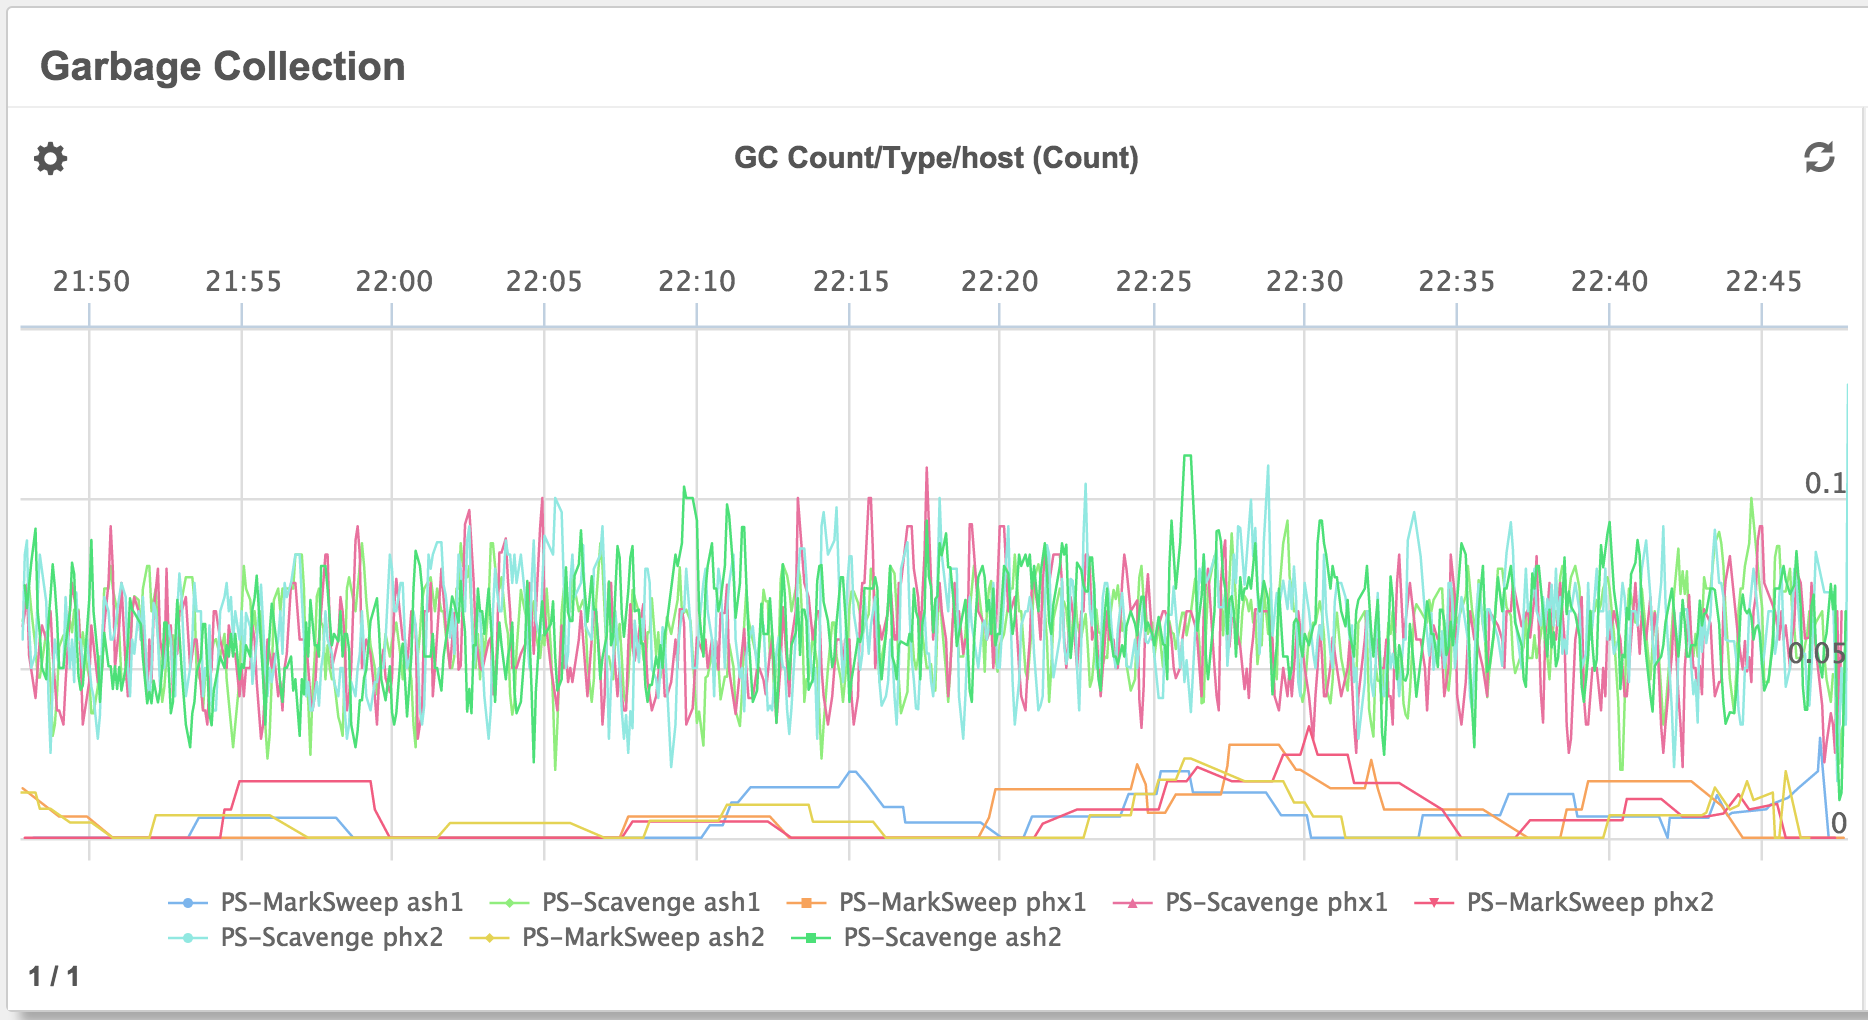
\includegraphics[width=0.8\textwidth]{images/metrilyx.png}
       \caption{Vizualizácia časových rád OpenTSDB pomocou Metrilyx}\cite{Metrilyx}
\end{center}
\end{figure}

\section{InfluxDB}
InfluxDB je platforma na zbieranie, uchovávanie, vizualizáciu a správu časových dát. Užívateľ môže vytvoriť viacero databáz. Dáta sa zapisujú a čítajú pomocou rozhrania príkazového riadka, 
rôznych klientskych knižníc, alebo pomocou HTTP API. Na vizualizáciu dát používa modul \emph{chronograf}.

\subsection{Politiky udržiavania}
Každá databáza obsahuje pravidlá, ktoré definujú, po akú dobu majú byť ukladané dáta časových rád a koľko kópií dát má byť vytvorených. Jedna databáza môže mať niekoľko takýchto politík. Pri zápise 
do nej je môžné špeicifikovať, ktorá politika sa má pre zápis použiť. Pri vytvorení databázy je automaticky vytvorená jedna politika

\subsection{Kontinuálne dotazovanie}
Databáza je schopná periodicky vykonávať požiadavky na dáta. Cieľom je zmenšovanie objemu dát. Ide o zhlukovanie dát s vysokou frekvenciou zberu, čím vzniknú dáta s menšou hustotou zberu. Táto hodnota je 
potom zvyčajne uložená do inej databázy.

\section{RRDTool}
RRDTool je nástroj na uchovávanie, spravovanie a vizuálizáciu časových dát. Využíva round-robin databázu. Je to databáza s dopredu danou maximálnou veľkosťou. V prípade, že príde požiadavka na zápis hodnoty 
a databáza je už plná, dôjde k prepisu nasjtaršej hodnoty. Tento nástroj takisto obsahuje funkcie na konsolidáciu dát. Konsolidovaná hodnota je typicky priemer, minimum alebo maximum z viacerých hodnôt zozbieraných 
za dlhší časový úsek. Tieto hodnoty sú ukladané do round-robin archívu.

\chapter{Aktuálne monitorovacie riešenia}
\section{Open-source}
\subsection{Nagios}
\subsubsection{PluginAPI}
Scripts and executables must do two things (at a minimum) in order to function as Nagios plugins:

Exit with one of several possible return values
Return at least one line of text output to STDOUT
The inner workings of your plugin are unimportant to Nagios. Your plugin could check the status of a TCP port, run a database query, check disk free space, or do whatever else it needs to check something. The details will depend on what needs to be checked - that's up to you.

Return Code

Nagios determines the status of a host or service by evaluating the return code from plugins. The following tables shows a list of valid return codes, along with their corresponding service or host states.

Plugin Return Code	Service State	Host State
\\0	OK	UP
\\1	WARNING	UP or DOWN/UNREACHABLE*
\\2	CRITICAL	DOWN/UNREACHABLE
\\3	UNKNOWN	DOWN/UNREACHABLE
\\Note Note: If the use\_aggressive\_host\_checking option is enabled, return codes of 1 will result in a host state of DOWN or UNREACHABLE. Otherwise return codes of 1 will result in a host state of UP. The process by which Nagios determines whether or not a host is DOWN or UNREACHABLE is discussed here.

Plugin Output Spec

At a minimum, plugins should return at least one of text output. Beginning with Nagios 3, plugins can optionally return multiple lines of output. Plugins may also return optional performance data that can be processed by external applications. The basic format for plugin output is shown below:

\\TEXT OUTPUT | OPTIONAL PERFDATA
\\LONG TEXT LINE 1
\\LONG TEXT LINE 2
\\...
\\LONG TEXT LINE N | PERFDATA LINE 2
\\PERFDATA LINE 3
\\...
\\PERFDATA LINE N

The performance data (shown in orange) is optional. If a plugin returns performance data in its output, it must separate the performance data from the other text output using a pipe (|) symbol. Additional lines of long text output (shown in blue) are also optional.
\cite{01}

\subsubsection{Timeouty}

Format:	service\_check\_timeout=<seconds>
Example:	service\_check\_timeout=60
This is the maximum number of seconds that Nagios will allow service checks to run. If checks exceed this limit, they are killed and a CRITICAL state is returned. A timeout error will also be logged.

There is often widespread confusion as to what this option really does. It is meant to be used as a last ditch mechanism to kill off plugins which are misbehaving and not exiting in a timely manner. 
It should be set to something high (like 60 seconds or more), so that each service check normally finishes executing within this time limit. If a service check runs longer than this limit, N
agios will kill it off thinking it is a runaway processes.

\cite{02}


Nie je mechanizmus pre reštart alebo individuálne timeouty.
Má zastaralý Hadoop plugin, používa staré REST API.
Last Release Date 2010-11-05
\cite{03}

\subsection{Zabbix}
\subsubsection{Timeouty}
Timeout processing
Zabbix will not process a simple check longer than Timeout seconds defined in Zabbix server configuration file.
\cite{04}

Zabbix Agent
Timeout	 no	 1-30	3	Spend no more than Timeout seconds on processing
\cite{20}

Zabbix Server
Timeout	 no	 1-30	3	Specifies how long we wait for agent, SNMP device or external check (in seconds).
\cite{05}

Neuvádza sa nič o zastavovaní procesov.
\subsubsection{Moduly}

Loadable modules offer a performance-minded option for extending Zabbix functionality.

There already are ways of extending Zabbix functionality by way of:

user parameters (agent metrics)
external checks (agent-less monitoring)
system.run[] Zabbix agent item.
They work very well, but have one major drawback, namely fork(). Zabbix has to fork a new process every time it handles a user metric, which is not good for performance. It is not a big deal normally, however it could be a serious issue when monitoring embedded systems, having a large number of monitored parameters or heavy scripts with complex logic or long startup time.

Zabbix 2.2 comes with support of loadable modules for extending Zabbix agent, server and proxy without sacrificing performance.

A loadable module is basically a shared library used by Zabbix daemon and loaded on startup. The library should contain certain functions, so that a Zabbix process may detect that the file is indeed a module it can load and work with.

Loadable modules have a number of benefits. Great performance and ability to implement any logic are very important, but perhaps the most important advantage is the ability to develop, use and share Zabbix modules. It contributes to trouble-free maintenance and helps to deliver new functionality easier and independently of the Zabbix core code base.
\cite{06}

\subsection{Icinga}
By default the Icinga 2 daemon is running as icinga user and group using the init script. Using Debian packages the user and group are set to nagios for historical reasons.
\cite{07}

\subsubsection{Externé pluginy}
Icinga determines the status of a host or service by evaluating the return code from plugins. The following tables shows a list of valid return codes, along with their corresponding service or host states
\cite{08}

\subsubsection{Notifikácie a príkazy udalostí}
Unlike notifications, event commands for hosts/services are called on every check execution if one of these conditions match:
The host/service is in a soft state
The host/service state changes into a hard state
The host/service state recovers from a soft or hard state to OK/Up

Ide len o spustenie nejakého systémového príkazu.
\cite{09}

\subsubsection{Itegrácie s aplikáciami} 
these tiny pure shell+awk plugins for monitoring your hadoop cluster are a enhanced and uptodate version of exchange.nagios.org check\_hadoop-dfs.sh
\cite{10}

\subsection{Cacti}
Cacti is a complete network graphing solution designed to harness the power of RRDTool's data storage and graphing functionality. Cacti provides a fast poller, advanced graph templating, multiple data acquisition methods, and user management features out of the box.
\cite{11}

\subsection{collectd}
There are some key differences we think set collectd apart. For one, it's written in C for performance and portability, allowing it to run on systems without scripting language or cron daemon, such as embedded systems. 
At the same time it includes optimizations and features to handle hundreds of thousands of data sets. It comes with over 90 plugins. It provides powerful networking features and is extensible in numerous ways. 

\subsubsection{Obmedzenia}
It does not generate graphs. It can write to RRD files, but it cannot generate graphs from these files. 
Monitoring functionality has been added in version 4.3, but is so far limited to simple threshold checking. 
\cite{12}

\subsubsection{Zapisovací plugin Write TSDB}
The Write TSDB plugin writes metrics to OpenTSDB, an open-source distributed time-series database based on Apache HBase.
\cite{13}

\begin{description}
\item[\emph{Host Address}] Hostname or address to connect to. Defaults to localhost.
\item[\emph{Port Service}] Service name or port number to connect to. Defaults to 4242.
\item[\emph{HostTags String}] When set, HostTags is added to the end of the metric. It is intended to be used for name=value pairs that the TSD will tag the metric with. Dots and whitespace are not escaped in this string.
\item[\emph{StoreRates false|true}] If set to true, convert counter values to rates. If set to false (the default) counter values are stored as is, as an increasing integer number.
\item[\emph{AlwaysAppendDS false|true}] If set the true, append the name of the Data Source (DS) to the "metric" identifier. If set to false (the default), this is only done when there is more than one DS.
\end{description}

\subsubsection{Prahy a notifikácie}

The only action the Threshold plugin takes itself is to generate and dispatch a notification. Every time a value is out of range, 
notification is dispatched. 
Also, all values that match a threshold are considered to be relevant or "interesting". As a consequence collectd will issue a notification 
if they are not received for Timeout iterations.  for example, Timeout is set to "2" (the default) and some hosts sends it's CPU statistics to the server every 60 seconds, a notification will be dispatched after about 120 seconds. It may take a little longer because the timeout is checked only once each Interval on the server.

When a value comes within range again or is received after it was missing, an "OKAY-notification" is dispatched.
\cite{14}

\subsection{Ostatne} 
\begin{description}
\item[\emph{Zenoss}]
\item[\emph{Munin}]
\end{description}

\section{Ganglia} 
Ganglia is a scalable distributed monitoring system for high-performance computing systems such as clusters and Grids. It is based on a hierarchical design targeted at federations of clusters. It leverages widely used technologies such as XML for data representation, XDR for compact, portable data transport, and RRDtool for data storage and visualization. It uses carefully engineered data structures and algorithms to achieve very low per-node overheads and high concurrency. The implementation is robust, has been ported to an extensive set of operating systems and processor architectures, and is currently in use on thousands of clusters around the world. It has been used to link clusters across university campuses and around the world and can scale to handle clusters with 2000 nodes.
Ganglia is a BSD-licensed open-source project that grew out of the University of California, Berkeley Millennium Project
\cite{15}
Pre Gangliu je dostupný monitorovací plugin pre Hadoop.
\cite{16}

\section{Komerčné riešenia}

\section{Torque}
Nenašiel som žiadne komerčný softvér na monitorovanie Torque. 

\section{libvirt/KVM}

\section{Docker}
\subsection{Scout}
Scout runs within Docker containers without any special configuration. \cite{scout}

\subsection{New Relic}
http://newrelic.com/docker

\subsection{AppDynamics}
https://www.appdynamics.com/community/exchange/extension/docker-monitoring-extension/


\section{Hadoop}
\subsection{New Relic}
http://newrelic.com/plugins

\subsection{AppDynamics}
The Hadoop monitoring extension captures metrics from Hadoop Resource Manager and/or Apache Ambari and displays them in Appdynamics Metric Browser.

This extension works only with the standalone machine agent.


Metrics include:

Hadoop Resource Manager
App status and progress: submitted, pending, running, completed, killed, and failed app count
Memory size, memory usage
Allocated containers, container count in different states
Node status, count of nodes in different states
Scheduler capacity, app and container count
Ambari
Individual host metrics including CPU, disk, memory, JVM, load, network, process, and RPC metrics
Service component metrics including CPU, disk, memory, JVM, load, network, process, RPC, and component-specific metrics
\cite{17}

\chapter{Cloudové technológie}

\section{Aplikačné kontajnery}
Kontajnery predstavujú odlišný prístup k virtualizácií ako virtuálne stroje. Tiež ide o snahu spúšťať softvér v prostredí oddelenom od skutočného hardvéru a operačného systému. Na rozdiel od úplných virtuálnych strojov 
nie je virtualizovaný celý hardvér, ale len softvérové vybavenie nevyhnutné na spustenie programu. Rozdiel v architektúre ilustruje nasledovný obrázok: 
\begin{figure}[h]
\begin{center}
       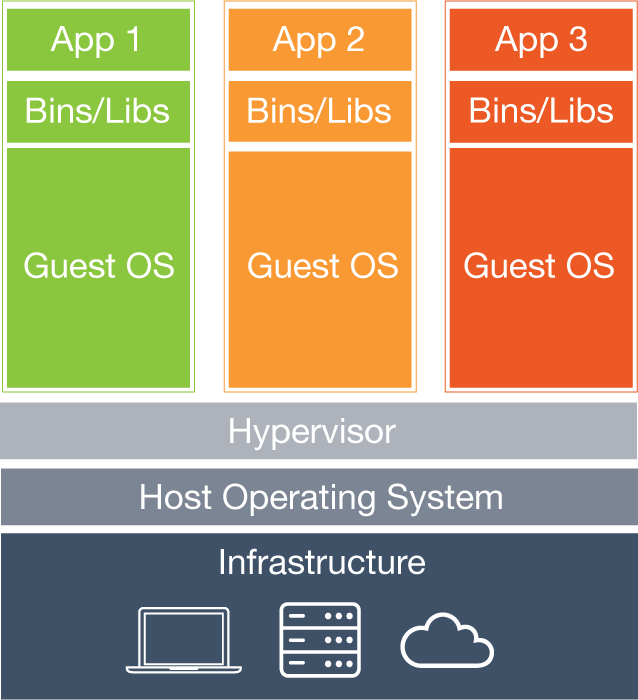
\includegraphics[width=0.8\textwidth]{images/docker.png}
       \caption{Porovnanie architektúry Docker a virtuálnych strojov}\cite{docker}
\end{center}
\end{figure}
V kontajneri môže byť spustený nezávislý operačný systém spolu s požadovanými aplikáciami. Hosťovský počítač, na ktorom sú kontajnery spustené, má jeden operačný systém a jednu množinu prostriedkov, 
ktoré tieto kontajnery zdieľajú. Jednotlivé kontajnery dostávajú kontrolovaný prístup k výpočtovému výkonu, pamäti, úložnej kapacite, sieti a prípadne ďalším prostriedkom.

\subsection{Linux cgroups}
Linux cgroups je technológia linuxového jadra, ktorá umožňuje limitovať, sledovať a izolovať spotrebu prostriedkov systému jednotlivými procesmi. Zavádza stromovo organizované kontrolné skupiny. 
Kontrolná skupina obsahuje obmedzenia pre jeden systémový prostriedok, tzv. susbsystém. Príklad subsystémov, ktoré poskytuje Red Hat Enterprise Linux: 
\begin{description}
\item[\emph{blkio}] - this subsystem sets limits on input/output access to and from block devices such as physical drives (disk, solid state, USB, etc.).
\item[\emph{cpu}] - this subsystem uses the scheduler to provide cgroup tasks access to the CPU.
\item[\emph{cpuacct}] - this subsystem generates automatic reports on CPU resources used by tasks in a cgroup.
\item[\emph{cpuset}] - this subsystem assigns individual CPUs (on a multicore system) and memory nodes to tasks in a cgroup.
\item[\emph{devices}] - his subsystem allows or denies access to devices by tasks in a cgroup.
\item[\emph{freezer}] - this subsystem suspends or resumes tasks in a cgroup.
\item[\emph{memory}] - this subsystem sets limits on memory use by tasks in a cgroup, and generates automatic reports on memory resources used by those tasks.
\item[\emph{net\_cls}] - this subsystem tags network packets with a class identifier (classid) that allows the Linux traffic controller (tc) to identify packets originating from a particular cgroup task.
\item[\emph{net\_prio}] - this subsystem provides a way to dynamically set the priority of network traffic per network interface.
\item[\emph{ns}] - the namespace subsystem.
\end{description}

Pre každý subsystém existuje jeden strom kontrolných skupín. Ďalej skupina obsahuje zoznam procesov, ktoré podliehajú definovaným obmedzeniam. V strome kontrolných skupín sa proces vyskystuje len raz.
V cloudovom prostredí však jednotlivé technológie využívajú a spúšťajú mnoho procesov,ktoré by sa obtiažne priraďovalo jednotlivým užívateľom v súvislosti so spustenými aplikáciami, preto tento spôsob
monitorovania nie je úplne vhodný.


\subsection{Docker}
Docker umožňuje zabaliť aplikáciu so všetkými jej závislosťami do štandardizovanej jednotky (tzv. kontajnery) určenej na softvérový vývoj. Kontajnery Dockeru obaľujú softvér kompletným súborovým systémom, ktorý
zahŕňa všetko, čo daný softvér potrebuje na spustenie: kód, nástroje potrebné na beh, systémové nástroje a knižnice. Toto zaručuje, že program bude pracovať rovnako bez ohľadu na prostredie, v ktorom
je spustený.\cite{docker}


\section{Virtuálne stroje}
Virtuálne stroje poskytujú úplnú virtualizáciu. Na jednom hosťujúcom počítači môže byť spustených viacero virtuálnych strojov. Každý má svoj vlastný virtuálny procesor, pamäť, grafický procesor, pevný disk 
a periférie. Operačný systém spustený vo virtuálnom stroji je izolovaný od hosťovského opračného systému (ak ho hosťovský počítač má). Takéto riešenie má jednu bezpečnostnú výhodu oproti aplikačným 
kontajnerom. Nežiadúce fungovanie jedného virtuálneho stroja neovplyvňuje beh ostatných.
V súčasnosti existuje mnoho úrovní virtuálnych strojov. Emulácia inštrukčnej sady, prekladanie programov za beho a ich optimalizácia, vysokoúrovňové virtuálne stroje (napr. Java) a systémové virtuálne stroje používané ako
jednotlivcami tak na serveroch.

\subsection{Hypervízor}
Hypervízor je softvér, ktorý vytvára a zabezpečuje beh virtuálnych strojov. Rozlišujeme 2 typy:
\begin{description}
\item[natívny] - na hosťujúcom počítači nie je nainštalovaný žiadny operačný systém. Hypervízor spravuje hardvér hosťujúceho počítača a kontroluje beh operačných systémov, ktoré sa javia ako procesy.
Príkladom je VMware ESX/ESXi, Oracle VM Server for x86 alebo Citrix XenServer.
\item[hosťovaný] - hypervízor je spustený ako bežný program v operačnom systéme hosťujúceho počítača. Príkladom je QEMU, VMware Workstation alebo VirtualBox.
\end{description}
\cite{hypervisorTypes}

\subsection{libvirt/KVM}
KVM\footnotemark\footnotetext{Kernel-based Virtual Machine} je plné virtualizačné riešenie pre Linux pre x86 hardvér, obsahujúce virtualizačné rozšírenia (Intel VT or AMD-V).
Pozostáva z nahrateľného modulu jadra, kvm.ko, ktorý poskytuje základ virtualizačnej infraštruktúry a šepcifický modul, kvm-intel.ko alebo kvm-amd.ko. Je možné virtualizovať obrazy 
s operačným systémami Linux aj Windows. Každý virtuálny stroj má vlastný virtualizovaný hardvér: sieťovú kartu, disk, grafický adaptér, atď. KVM je open-source softvér. Virtualizačný modul jadra
sa nachádza v Linuxe od verzie 2.6.20.\cite{kvm}

libvirt je sada nástrojov na prácu s virtualizačnými schopnosťami Linuxu (a ostatných OS). Je to voľný softvér dostupný pod licenciou GNU LGPL. 
Obsahuje API v jazyku C a väzby pre bežné programovacie jazyky.\cite{libvirt}


\section{MapReduce aplikačné prostredia}
\subsection{Hadoop}
Projekt Apache Hadoop vyvíja open-source softvér na spoľahlivé, škálovateľné, distribuované výpočty. Apache Hadoop je prostredie, ktoré umožňuje distribuované spracovávanie veľkých množstiev dát
naprieč clustermi, používajúcimi jednoduché programovacie modely. Je navrhnutý tak, aby bol škálovateľný od jednotlivých serverov po tisícky strojov, kde každý poskytuje lokálny výpočetný výkon a úložný priestor.
Nespolieha sa na vysokú dosupnosť hardvérových prostriedkov, ale je navrhnutý, aby detekoval a zvládal chyby na aplikačnej vrstve, takže poskytuje vysoko dostupnú službu nad clusterom počítačov, 
z ktorých každý je náchylný na chyby.

Projekt pozostáva z týchto modulov:
\begin{description}
\item[\emph{Hadoop Common:}] spoločné nástroje, ktoré podporujú ostatné Hadoop moduly
\item[\emph{Hadoop Distributed File System (HDFS™):}] distribuovaný súborový systém, ktorý poskytuje vysokú priepustnosť
\item[\emph{Hadoop YARN:}] prostredie pre plánovanie úloh a správu zdrojov clustera
\item[\emph{Hadoop MapReduce:}] systém založený na YARN pre paralelné spracovávanie veľkých množstiev dát, prostredie pre plánovanie úloh a správu zdrojov clustera
\end{description}

\chapter{Metriky}
Každá z technolóǵií cloudového výpočetného strediska je zdrojom mnohých dát o vyťažení zdrojov. Je potrebné určiť, ktoré zdroje monitorovať a ktoré metriky zberať. Je vhodné mať také metriky pre všetky využívané cloudové technológie, ktoré je možné
nejakým spôsobom porovnať medzi sebou. V prípade procesora sa jedná o jeho aktuálne vyťaženie, ale zároveň je zaujímavým údajom aj prepočítaný procesorový čas. Táto metrika môže byť efektívnym
nástrojom pre následné učtovanie jednotlivým úžívateľom. Keďže majú ale tieto technológie principiálny rozdiel vo svojom určení, nie je možné vždy o každom zdroji zberať rovnaké dáta. 
O distribuovaných výpočtoch napríklad nie je možné efektívne zistiť aktuálne vyťaženie procesora. Takéto úlohy sa počítajú na viacerých uzloch clustera. O poradí a rozmiestnení požiadaviek na zdroje
rozhodouje riadiaca aplikácia, takže sa nejedná o jeden procesor. Táto aplikácia má ale prehľad o tom, koľko času strávil celý cluster počítaním danej úlohy. Takže v určitom ohľade zrovnateľná s virtuálnym
strojom a jeho spotrebou procesorového času.

Podobná situácia nastáva aj u monitorovania sieťových rozhraní. Distribuované výpočty využívajú sieť svojským spôsobom a len na účel vypočítania komplexnejšieho problému. Jedná sa o prepojenie
uzlov v rámci clustera. Je to jednoúčelová vysokorýchlostná sieť. Z hľadiska poskytovania výpočetných kapacít dáva väčší zmysel orientácia na využívanie konektivity smerom do internetu. 

\subsection{Význam popisných údajov metrík}
Metrické dáta vypovedajú o využití zdrojov. Vieme určiť ako dlhý čas a v akej miere bol využívaný výpočtový výkon. Z nich samotných nevieme presne určiť, kto zdroje využíval. Pre to aby mali tieto dáta zmysel 
pre neskoršie účtovanie, je potrebné mať možnosť ich priradiť k užívateľom, či už sa jedná o vlastnika virtuálneho stroja alebo uživateľa, ktorý spustil kontrétnu úlohu. Na základe týchto ďalších popisných  údajov je potom 
možné zisťovať, kto zdroje vyťažoval za časové obdobie najviac a podľa toho stanoviť prípadnú cenu za používanie zdrojov. Okrem identity je vhodné metriky popisovať aj ďalšími údajmi, ako je miesto, kde
sa zdroj nachádza, názov stroja, ktorý poskytuje svoje kapacity, a ďalšie špecifické údaje, ktoré sa týkajú jednotlivých technológií, ktoré budem popisovať konkrétnejšie v ďalších častiach.

\subsection{Periodicita zberania metrík}
Zberané metriky sa líšia tým, ako veľmi sa v čase menia. Kým záťaž procesora, vstupno-výstupné operácie alebo množstvo prenesených dát sa mení v čase pomerne rýchlo, veľkosť clustera v počte poskytnutých procesorov 
alebo virtuálnej pamäte sa nemení tak často. Má preto zmysel uvažovať o kontrole intervalu zbierania jednotlivých metrík. Nie len 
na úrovni zhluku metrík pre konrétnu technológiu ale aj pre jednotlivé metriky samostatne.

\subsection{Formát hodnoty metriky}
Metriky ako záznamy obsahujú čas, kedy bola hodnota nameraná, samotnú hodnotu nejakého sledovaného javu a popisné dáta. Na metrické
hodnoty sa môžeme pozerať ako na prírastky alebo ako na absolútne hodnoty. Prírastky hovoria o rozdiele aktuálne nameranej hodnoty 
a poslednej hodnoty. Absolútne hodnoty predstavujú aktuálnu nameranú hodnotu využitia zdroja. 

\section{Docker}
\subsection{Sieť}
Aby mohli medzi sebou jednotlivé kontajnery komunikovať, Docker im poskytuje sieťové rozhrania. Každé rozhranie má nakonfigurovanú sieť,
do ktorej patrí. Na to, aby kontajnery spolu mohli komunikovať, musia byť členmi rovnakej siete. Komunikácia naprieč sieťami nie je možná.
Užívatelia si môžu definovať vlastné siete. Docker na vytvorenie týchto sietí poskytuje dva ovládače.

\subsubsection{Sieť typu most}
Je to jednoduchý typ siete určený pre malé siete. Je ju možné vytvoriť príkazom 
\\
{\em \$ docker network create --driver bridge NÁZOV\_SIETE}
\\ \\
Po vytvorení siete je možné spustiť kontajnery v tejto sieti príkazom
\\ \\
{\em \$ docker run --net=NÁZOV\_SIETE --name=NÁZOV\_KONTAJNERA}

\subsubsection{Prekladaná sieť}
Docker umožňuje vytvoriť aj sieť, v ktorej sa nachádza viacero hosťujúcich počítačov zároveň. To umožňuje komunikovať medzi sebou aj kontajnerom,
ktoré sú spustené v rozličných sieťach, prípadne na inom hosťujúcom počítači..


\subsubsection{Metriky siete}
Pre jednotlivé sieťové rozhrania je možné zbierať tieto metriky:
\begin{description}
\item[rx\_bytes] - počet prijatých bajtov
\item[rx\_dropped] - počet prichádzajúcich zahodených bajtov
\item[rx\_error] - počet chybných bajtov
\item[rx\_packets] - počet prijatých paketov
\item[tx\_bytes] - počet odoslaných bajtov
\item[tx\_dropped] - počet zahodených bajtov pri pokuse o odoslanie
\item[tx\_errors] - počet odoslaných chybných bajtov
\item[tx\_packets] - počet odoslaných paketov
\end{description}

\subsection{Pamäť}
Cez API Dockeru je možné získať nasledovné metriky pamäte.
\begin{description}
\item[usage] - spotreba pamäte
\item[failcnt] - počet chýb
\end{description}
Docker neposkytuje údaj o tom, koľko pamäte poskytuje hosťujúci počítač. Zistiť tento údaj však v implementácií nepredstavuje problém,
a preto je tiež zberaná táto metrika.

\subsection{Procesor}
Procesor predstavuje jeden z najdôležitejších údajov o vyťažení zdrojov. Docker poskytuje viaceré metriky o procesore, ktorých hodnoty 
predstavujú výpočetný čas strávený na procesore: 
\begin{description}
\item[percpu\_usage] - využitie jednotlivých jadier procesora
\item[usage\_in\_usermode] - 
\item[total\_usage] - 
\item[usage\_in\_kernelmode] - 
\item[system\_cpu\_usage] - 
\end{description}

\section{libvirt/KVM}

\subsection{Metriky siete}
Pre jednotlivé sieťové rozhrania je možné zbierať tieto metriky:
\begin{description}
\item[rx\_bytes] - počet prijatých bajtov
\item[rx\_dropped] - počet prichádzajúcich zahodených bajtov
\item[rx\_error] - počet chybných bajtov
\item[rx\_packets] - počet prijatých paketov
\item[tx\_bytes] - počet odoslaných bajtov
\item[tx\_dropped] - počet zahodených bajtov pri pokuse o odoslanie
\item[tx\_errors] - počet odoslaných chybných bajtov
\item[tx\_packets] - počet odoslaných paketov
\end{description}

\subsection{Metriky pamäte}
\begin{description}
\item[VIR\_DOMAIN\_MEMORY\_STAT\_SWAP\_IN] - The total amount of memory written out to swap space (in kB).
\item[VIR\_DOMAIN\_MEMORY\_STAT\_SWAP\_OUT] - Page faults occur when a process makes a valid access to virtual memory that is not available. When servicing the page fault, if disk IO is required, it is considered a major fault. If not, it is a minor fault. These are expressed as the number of faults that have occurred.
\item[VIR\_DOMAIN\_MEMORY\_STAT\_MAJOR\_FAULT] - počet chybných bajtov
\item[VIR\_DOMAIN\_MEMORY\_STAT\_MINOR\_FAULT] - počet prijatých paketov
\item[VIR\_DOMAIN\_MEMORY\_STAT\_UNUSED] - The amount of memory left completely unused by the system. Memory that is available but used for reclaimable caches should NOT be reported as free. This value is expressed in kB.
\item[VIR\_DOMAIN\_MEMORY\_STAT\_AVAILABLE] - The total amount of usable memory as seen by the domain. This value may be less than the amount of memory assigned to the domain if a balloon driver is in use or if the guest OS does not initialize all assigned pages. This value is expressed in kB.
\item[VIR\_DOMAIN\_MEMORY\_STAT\_ACTUAL\_BALLOON] - Current balloon value (in KB).
\item[VIR\_DOMAIN\_MEMORY\_STAT\_RSS] - Resident Set Size of the process running the domain. This value is in kB
\item[VIR\_DOMAIN\_MEMORY\_STAT\_NR] - The number of statistics supported by this version of the interface. To add new statistics, add them to the enum and increase this value.
\end{description}

\subsection{Metriky zápisu dát}
\begin{description}
\item[rd\_req] - number of read requests
\item[rd\_bytes] - number of read bytes
\item[wr\_req] - number of write requests
\item[wr\_bytes] - number of written bytes
\item[errs] - In Xen this returns the mysterious 'oo\_req'.
\end{description}

\subsection{Metriky CPU}
Libivirt poskytuje o procesore údaj o tom, koľko výpočetného času strávil daný virtuálny stroj na procesore hosťujúceho počítača.


\section{Hadoop}
\subsection{Cluster Metrics API}
Toto API poskytuje metriky o celom clusteri.
\begin{description}
\item[appsSubmitted] - The number of applications submitted
\item[appsCompleted] - The number of applications completed
\item[appsPending] - The number of applications pending
\item[appsRunning] - The number of applications running
\item[appsFailed] - The number of applications failed
\item[appsKilled] - The number of applications killed
\item[reservedMB] - The amount of memory reserved in MB
\item[availableMB] - The amount of memory available in MB
\item[allocatedMB] - The amount of memory allocated in MB
\item[totalMB] - The amount of total memory in MB
\item[reservedVirtualCores] - The number of reserved virtual cores
\item[availableVirtualCores] - The number of available virtual cores
\item[allocatedVirtualCores] - The number of allocated virtual cores
\item[totalVirtualCores] - The total number of virtual cores
\item[containersAllocated] - The number of containers allocated
\item[containersReserved] - The number of containers reserved
\item[containersPending] - The number of containers pending
\item[totalNodes] - The total number of nodes
\item[activeNodes] - The number of active nodes
\item[lostNodes] - The number of lost nodes
\item[unhealthyNodes] - The number of unhealthy nodes
\item[decommissionedNodes] - The number of nodes decommissioned
\item[rebootedNodes] - The number of nodes rebooted
\end{description}

\subsection{Cluster Application API}
Tento koncový bod API poskytuje informácie o jednotlivých aplikáciách, ktoré boli alebo sú spustené na clusteri.
\begin{description}
\item[id] - The application id
\item[user] - The user who started the application
\item[name] - The application name
\item[Application Type] - The application type
\item[queue] - The queue the application was submitted to
\item[state] - The application state according to the ResourceManager - valid values are members of the YarnApplicationState enum: NEW, NEW\_SAVING, SUBMITTED, ACCEPTED, RUNNING, FINISHED, FAILED, KILLED
\item[finalStatus] - The final status of the application if finished - reported by the application itself - valid values are: UNDEFINED, SUCCEEDED, FAILED, KILLED
\item[progress] - The progress of the application as a percent
\item[trackingUI] - Where the tracking url is currently pointing - History (for history server) or ApplicationMaster
\item[trackingUrl] - The web URL that can be used to track the application
\item[diagnostics] - Detailed diagnostics information
\item[clusterId] - The cluster id
\item[startedTime] - The time in which application started (in ms since epoch)
\item[finishedTime] - The time in which the application finished (in ms since epoch)
\item[elapsedTime] - The elapsed time since the application started (in ms)
\item[amContainerLogs] - The URL of the application master container logs
\item[amHostHttpAddress] - The nodes http address of the application master
\item[allocatedMB] - The sum of memory in MB allocated to the application’s running containers
\item[allocatedVCores] - The sum of virtual cores allocated to the application’s running containers
\item[runningContainers] - The number of containers currently running for the application
\item[memorySeconds] - The amount of memory the application has allocated (megabyte-seconds)
\item[vcoreSeconds] - The amount of CPU resources the application has allocated (virtual core-seconds)
\end{description}

\subsection{Node Application API}
Toto API poskytuje metriky o využití jednotlivých uzlov clusteri.
\begin{description}
\item[rack] - The rack location of this node
\item[state] - State of the node - valid values are: NEW, RUNNING, UNHEALTHY, DECOMMISSIONED, LOST, REBOOTED
\item[id] - The node id
\item[nodeHostName] - The host name of the node
\item[nodeHTTPAddress] - The nodes HTTP address
\item[healthStatus] - The health status of the node - Healthy or Unhealthy
\item[healthReport] - A detailed health report
\item[lastHealthUpdate] - The last time the node reported its health (in ms since epoch)
\item[usedMemoryMB] - The total amount of memory currently used on the node (in MB)
\item[availMemoryMB] - The total amount of memory currently available on the node (in MB)
\item[usedVirtualCores] - The total number of vCores currently used on the node
\item[availableVirtualCores] - The total number of vCores available on the node
\item[numContainers] - The total number of containers currently running on the node
\end{description}

\chapter{Analýza a návrh}
\section{MetaCentrum}
Projekt MetaCentrum vznikol v roku 1996 a od roku 1999 je jeho činnosť zastrešovaná organizáciou CESNET. Zaoberá sa budovaním nárdonej gridovej infraštruktúry a prepojením s podobnými projektami za hranicami
Českej republiky. Projekt je oficiálnou súčasťou Európskej gridovej iniciatívy (EGI). Úlohou MetaCentra je predovšetkým koordinácia a rozširovanie infraštruktúry či už o vlastné zdroje alebo prostredníctvom
partnerov, ktorý poskytujú výpočetný výkon svojich clusterov. Jedná sa hlavne o akademickú spoluprácu. MetaCentrum spravuje výpočetné prostriedky a dátové úložiská AV, JČU, MU, MZLU, UK, VUT, ZČU.
V súčasnosti disponuje (stav k 30.7. 2010) 1500 jadrami CPU, 100 TB využiteľnej diskovej kapacity v podobe poľa a 400 TB kapacity v podobe pások. Služby využíva 385 registrovaných aktívnych užívateľov, ktorí 
spolu na 750 tisíc úlohách využili 7 miliónov hodín procesorového času.

MetaCentrum primárne poskytuje svoj výpočetný výkon a úložnú kapacitu. Taktiež sprístupňuje svoje programové vybavenie a vývojové prostredie a hlavne množstvo aplikácií využívaných na výskumné účely, ako napr. 
Ansys, Gaussian, Matlab, Mathematica. Taktiež sa venuje vývoju v oblasti gridového a cloudového počítania, napr. v oblasti plánovania, gridového middleware, optimalizácie a paralelizácie výpočtov a virtualizácie
infraštruktúry. Dôležitou funkciou je účasť na medzinárodných projektoch, využívanie medzinárodnej výpočetnej infraštruktúry a využívanie skúseností na rozvoj v domácom prostredí.

\section{Požiadavky na aplikáciu}
\subsection{Vysoký monitorovací výkon}
Cloudová infraštruktúra MetaCentra pozostáva z mnohých výpočetných uzlov. Sú prepojené sieťami s veľkou prenosovou kapacitou a vysokou priepustnosťou. Je potrebné zbierať dáta o využití množstva zapojených
clusterov, na ktorých je tiež spustených mnoho výpočetných úloh či virtuálnych strojov. Metriky sú zbierané periodicky v určitých intervaloch z jednotlivých uzlov. Veľká záťaž je kladená na databázu, do ktorej
sú tieto metrické dáta pravidelne odosielané.

\subsection{Nízka nadbytočná záťaž}
Primárnou úlohou cloudu je poskytovanie svojho výpočetného výkonu a prostriedkov. Je žiadúce, aby monitorovacia aplikácia predstavovala čo najmenšiu záťaž pre systémy, na ktorých je spustená. Ak by monitorovanie
samotné spotrebovávalo príliš veľa zdrojov, takto získané metriky by nemali požadovanú presnosť. Je to možné docieliť výberom efektívneho programovacieho jazyka, napr. C, C++, prípadne rýchle skriptovacie 
jazyky ako Python, Ruby či Go. Nie je príliš vhodné používať jazyky, ktoré na svoj beh potrebujú ďalšiu vrstvu v podobe virtuálneho stroja, ako napr. Java.

\subsection{Škálovateľnosť}
Monitorovacia aplikácia by mala poskytovať zrovnateľné výsledky v oblasti rýchlosti odozvy v prípade, že bude spustená na jednom uzle, ale aj v prípade, že jej úlohou bude monitorovať desiatky až stovky 
výpočetných uzlov s množstvom spustených aplikácií. To je možné docieliť vhodným paralelizovaním dotazov na metriky

Monitorovacia aplikácia bude pozostávať z dvoch častí.
\begin{description}
\item[démon] - jeho úlohou je zber metrík a odosielanie do databázy
\item[zásúvné moduly] - ich úlohou je zisťovanie metrických dát a odosielanie démonovi
\end{description}

Démon je program, ktorý je spustený raz a beží v systéme na pozadí. Podľa konfigurácie pri štarte zistí, ktoré moduly sa budú používať. Takisto dôjde ku konfigurácií jednotlivých modulov, napr. nastavenie
potrebných ciest k požadovaným súborom. Následne dôjde k inicializácií jednotlivých modulov. V tejto fáze moduly inicializujú prostriedky, ktoré potrebujú v priebehu zberu metrík. Napr. pripojenie na správcu kontajnerov alebo hypervízora. Nie je efektívne, aby boli tieto prostriedky incializované pri
každej požiadavke na metriku, pretože by to spomaľovalo proces samotného zberu dát. Potom nasleduje fáza behu. Démon periodicky spúšťa jednotlivé moduly, ktoré zisťujú metrické dáta. Tie následne
vracajú ako odpoveď démonovi. V prípade, že je potrebné démona ukončiť, dôjde najprv k ukončeniu jednotlivých modulov. V tejto fáze moduly uvoľnia všetky prostriedky, ktoré mali naalokované.


\section{Reakcia na dlhú odozvu modulu}
Ak je hodnota nejakej metriky mimo určitý rozsah, je generované hlásenie. Na to je možné reagovať.
Na situáciu, keď časť zodpovedná za zbieranie dát neodpovedá, je ale možné reagovať len reštartovaním celej monitorovacej aplikácie. Nie je možné jednotlivé pluginy ovládať nezávisle. 

V princípe nejde nijako odlíšiť, či daný modul čaká na údaje alebo došlo k chybe a modul neodpovedá. Preto bude potrebné vytvoriť niektoré pluginy tak, aby jedna časť bola neustále dostupná 
a reagovala na výzvy od riadiacej aplikácie. Bude definovaný časový interval na vrátenie hodnoty. V prípade ak plugin úspešne v časovom intervale zistil dané metrické dáta, vráti ich riadiacej aplikácií. V prípade, že v danom intervale plugin neobdržal metrické dáta,
vráti poslednú hodnotu. Zároveň sa nebudú vytvárať nové požiadavky na tento údaj. Tento časový interval si bude môcť užívateľ nastaviť pre každú sondu. Predmetom testovania bude zistiť, 
aký interval by bol vhodný pre tú ktorú sondu.

Ďalšou prahovou hodnotou bude počet opakovaní, pri ktorých plugin vracia poslednú hodnotu danej metriky. Ak dôjde k prekročeniu tejto hodnoty, bude reštartovaná celá monitorovacia aplikácia.

\section{OpenTSDB}
Ako databázu na uchovávanie časových dát som si zvolil OpenTSDB. Dôvodom je používanie databázy HBase. Je to distribuovaná databáza určená pre veľké objemy dát v rádoch stoviek miliónov a milárd záznamov. 
Je typom NoSQL databázy. Oproti SQL databázam je linárne škálovateľná. Ak dôdje k zdvojnásobeniu výpočetných zdrojov, dôjde aj k zdvojnásobeniu výkonu databázy. To je dôležité pri zbere časových dát z mnohých uzlov,
ktoré sa v gridovej infraštruktúre MetaCentra nachádzajú. Ďalším dôvodom je, že v MetaCentre je aktuálne databáza HBase využívaná.


\chapter{Implementácia}
Využijem existujúcu aplikáciu na zbieranie metrických dát \emph{collectd}. Na zbieranie jednotlivých metrík som vytvoril moduly pre tento program. Tieto údaje následne bude odosielať do databázy OpenTSDB
pomocou modulu WriteTSDB.

\section{Techniky zbierania metrík}
\subsection{Torque}
Na zbieranie metrík som použil príkaz \emph{qstat -j}.

			Prints either for all pending jobs  or  the  jobs  contained  in  job\_list  various information. The job\_list
          can contain job\_ids, job\_names, or wildcard  expression
          sge\_types(1).

          For  jobs  in  E(rror)  state  the  error   reason   is
          displayed. For jobs that could not be dispatched during
          in the  last  scheduling  interval  the  obstacles  are
          shown, if 'schedd\_job\_info' in sched\_conf(5) is config-
          ured accordingly.

          For running  jobs  available  information  on  resource
          utilization   is  shown  about  consumed  cpu  time  in
          seconds,  integral  memory  usage  in  Gbytes  seconds,
          amount  of  data  transferred in io operations, current
          virtual memory utilization in Mbytes, and maximum  vir-
          tual  memory utilization in Mbytes. This information is
          not available if resource utilization retrieval is  not
          supported for the OS platform where the job is hosted.
          
\subsection{Docker}
Budem zberať metriky o spotrebovávaných zdrojoch pre každý kontajner. Na komunikáciu s Dockerom je možné využiť:
\begin{description}
\item[príkazy aplikácie v príkazovom riadku]
\item[Remote API]
\end{description}

Používanie príkazov aplikácie môže byť o čosi rýchlejšie, ale následne by bolo potrebné analyzovať textový výstup programu.
Rozhodol som sa použiť Remote API. Toto API funguje pre účely monitorovania na princípe REST a odpovede vracia vo formáte JSON, čo predstavuje zjednodušenie spracovania výstupu. Démon Dockeru "počúva" na 
lokálnom sockete, čo by nemalo spôsobovať výrazné oneskorenie odpovede.

O každom kontajneri spustenom v Dockeri budem sledovať využívanie týchto zdrojov :
\begin{description}
\item[\emph{procesor}]
\item[\emph{pevný disk}]
\item[\emph{sieť}]
\item[\emph{pamäť}]
\end{description}

  
Dáta je možné zberať buď ako prúd, alebo po jednorazových žiadostiach. To ešte nemám veľmi preštudované, neviem aké sú tam intervaly, tak sa rozhodnem až neskôr.
Predpokladám ale, že z hľadiska rýchlosti a alokácie bude cesta asi ten stream.

\subsection{libvirt/KVM}
Na monitorovanie virtuálnych strojov použijem existujúcu implementáciu sond v jazyku Python. Je šírená pod licenciou open-source a vznika v rámci organizácie Cesnet. 

\subsection{Hadoop}
The Hadoop YARN web service REST APIs are a set of URI resources that give access to the cluster, nodes, applications, and application historical information. 
The URI resources are grouped into APIs based on the type of information returned. Some URI resources return collections while others return singletons.
HTTP Requests

To invoke a REST API, your application calls an HTTP operation on the URI associated with a resource.

Summary of HTTP operations

Currently only GET is supported. It retrieves information about the resource specified.

Security

The web service REST API’s go through the same security as the web UI. 

\cite{18}



\chapter{Záver}

\bibliographystyle{csplainurl}
\nocite{*}
\bibliography{dip-lezdik}
\addcontentsline{toc}{chapter}{Literatúra}

\begin{appendix}
\chapter{Kapitola priloha}
\end{appendix}

\end{document}
